\documentclass[12pt,journal,compsoc]{IEEEtran}

\usepackage[english,portuguese]{babel}
\usepackage[utf8]{inputenc}
\usepackage[cmex10]{amsmath}
\usepackage{amssymb}
\usepackage{graphicx}
\usepackage[colorinlistoftodos]{todonotes}
\usepackage{tikz}
\usepackage{subfigure}
\usetikzlibrary{shapes, shadows, arrows}
\usepackage{float}
\usepackage{color}
\usepackage{hyperref}
\usepackage{fancyhdr}
\pagestyle{fancyplain}

\begin{document}

\title{Microcontroladores II -- Laboratório II \\ USART com API HAL}

\author{Prof. Francisco Granziera Júnior
\IEEEcompsocitemizethanks{\IEEEcompsocthanksitem 
Prof. Francisco Granziera Júnior é docente do Departamento de Engenharia Elétrica da Universidade Estadual de Londrina (UEL), Londrina, PR.\protect\\
E-mail: granziera@uel.br
%\IEEEcompsocthanksitem Ana García is Electrical Engineer student.
}
\thanks{Primeira versão 09/03/2022.}}

\markboth{1ELE910 -- Microcontroladores II}%
{\MakeLowercase{}Lab. I -- GPIO com API HAL}

\IEEEtitleabstractindextext{%
\begin{abstract}
Este laboratório tem por objetivo fazer uso da API HAL para implementações de tarefas envolvendo a GPIO e USART. 
\end{abstract}

\begin{IEEEkeywords}
API HAL, GPIO, USART, STM32F4DISC.
\end{IEEEkeywords}}

\maketitle

\IEEEdisplaynontitleabstractindextext

\IEEEpeerreviewmaketitle

\begin{flushright}
    {\textit{Uma pessoa que nunca cometeu um erro,\\
    nunca tentou nada novo.}\\
      \textbf{Albert Einstein (1879--1955)}}
\end{flushright} 

\section{Introdução}

{A} realização deste experimento irá requerer o uso de algumas ferramentas novas. Faremos uso do ambiente de desenvolvimento STM32CubeIDE da ST na sua última versão que pode ser baixado gratuitamente do site da fabricante. Esta ferramenta está integrada a uma outra, STM32CubeMX que permite a configuração \emph{wizard} do chip ou da placa de desenvolvimento. Para obter a ferramenta acesse o site \texttt{www.st.com}, efetue o login (faça o cadastro caso não tenha) e procure por STM32CubeIDE, que nesta data encontra-se na versão 1.8.0. Note que esta ferramenta está disponível para os sistemas operacionais mais comuns: Windows 10, iOS e Linux.

Uma segunda ferramenta que utilizaremos é o kit de desenvolvimento STM32F4DISC. Ele porta um microcontrolador ARM-Cortex M4 STM32F407VG com bastante recursos. Para expandir o acesso e uso de seus periféricos, utilizaremos a placa de expansão Open407V-D da WaveShare que possui uma enorme gama de \emph{shields} que podem ser acoplados a mesma.

A documentação do hardware é essencial e pode ser encontrada no site do fabricante. Por exemplo, da WaveShare \texttt{www.waveshare.com/wiki/Open407V-D}. Alguns arquivos principais foram selecionados na pasta Dropbox da disciplina e podem ser acessados em \texttt{encurtador.com.br/fHOR4}.

\section{Descrições Básicas}

\subsection{Recursos Necessários}

Para realização desta prática será necessário:

\begin{itemize}
\item Kit STM32F4DISC com STM32F407VG
\item Placa de expansão Open407V-D
\item Desktop com STM32CubeIDE instalado e atualizado.
\end{itemize}

\subsection{\emph{Mise en place des initiatives}}

Baixar a instalar o STM32CubeIDE é demorado (cerca de 45 minutos), portanto, caso faça uso de um notebook pessoal durante as aulas, instale com antecedência. 

Mesmo com o STM32CubeIDE instalado, ao fazer primeiro uso criando um projeto que selecione a board STM32F4DISC será feito o download ($\approx$ 900 MB) e instalações dos pacotes referentes à família e modelo do microcontrolador, isto também leverá um bom tempo (dependendo da velocidade da conexão com a internet) para ser concluído.

Note que ao criar um projeto com base em uma placa de desenvolvimento existe a opção de criar o projeto com todos os periféricos pré-configurados (CLOCKs, USART, I2C, BOT, LEDs, etc.). Esta opção é preferível, e caso algum periférico entre em conflito com nossa aplicação, podemos reconfigurá-lo.

A Fig. \ref{fig1} mostra o recurso gráfico para configuração dos pinos do microcontrolador. Ao clicar sobre um pino pode-se verificar ou modificar sua atribuição (entrada, saída, AF, etc.). 

\begin{figure}[!ht]
\centering
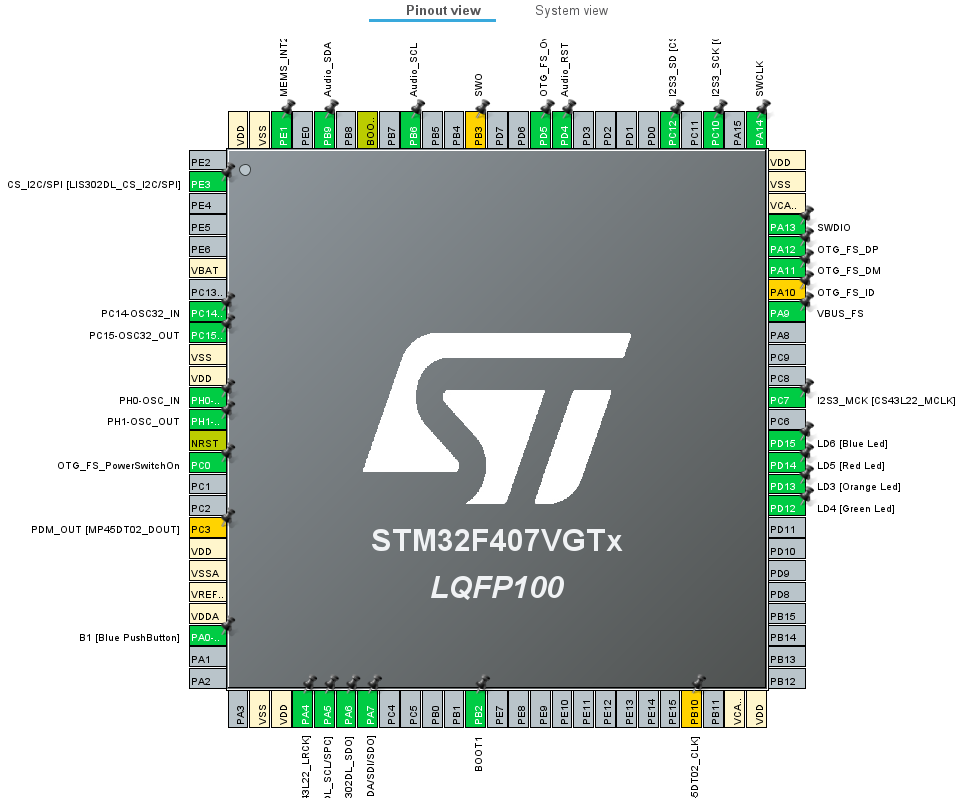
\includegraphics[trim = 0.0cm 0.0cm 0.0cm 0.0cm, clip, width=0.48\textwidth]{chip_01.png}
\caption{\label{fig1} Pinout view no STM32CubeIDE. Arquivo \texttt{.ioc}}
\end{figure}

Além disso, pode-se realizar qualquer configuração inicial de qualquer pino de GPIO e estas configurações serão incluídas da geração de código. Estas pré-configurações são possíveis também para os periféricos. Para o Clock, há uma aba exclusiva, como mostrado na Fig. \ref{fig2}. 

\begin{figure}[!ht]
\centering
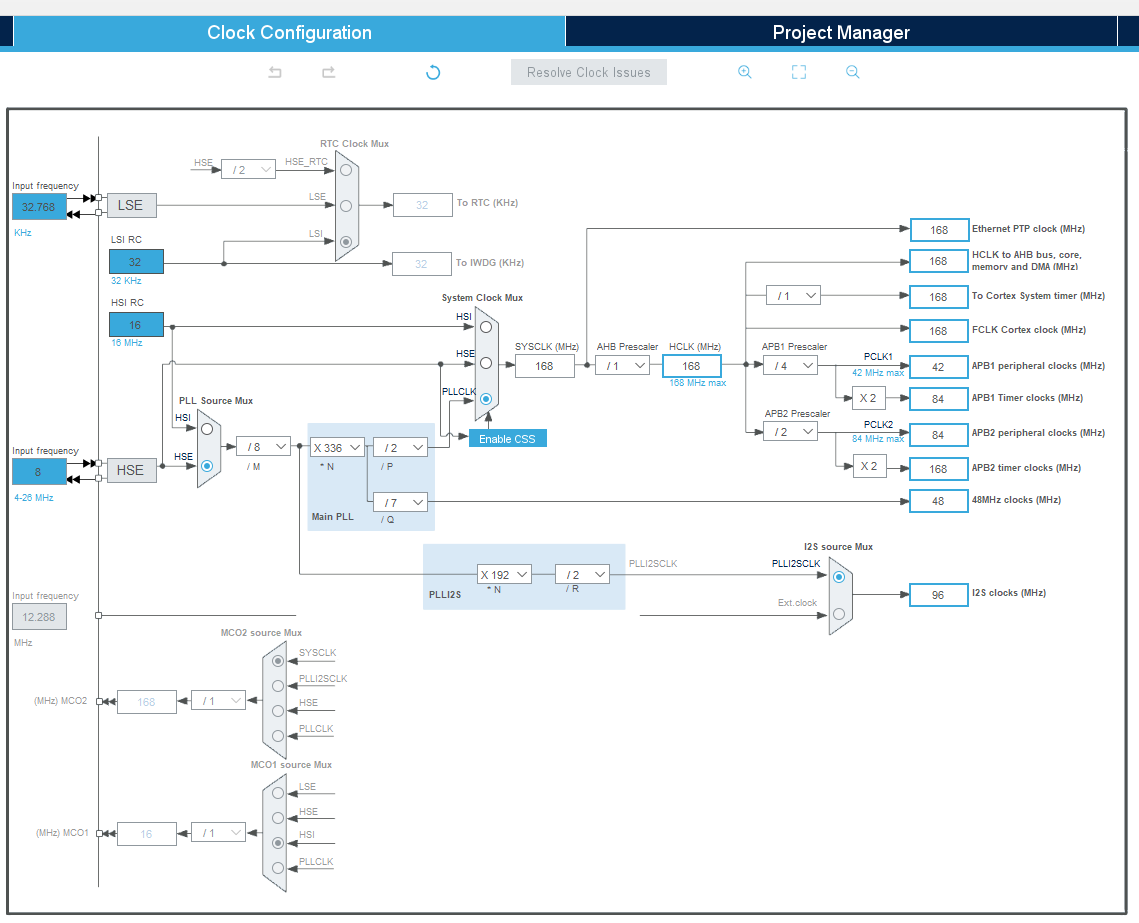
\includegraphics[trim = 0.0cm 0.0cm 0.0cm 0.0cm, clip, width=0.48\textwidth]{clock_01.png}
\caption{\label{fig2} Aba para configuração dos clocks.}
\end{figure}

\subsection{API HAL para GPIO: estruturas}

A API HAL para GPIO Genérica possui uma estrutura bem semelhante a da SPL (Standard Peripheral Library). Basicamente existem os seguintes campos de dados:

\begin{flushleft}
{\texttt{
\noindent\ignorespacesafterend
uint32\_t  Pin \\
uint32\_t  Mode \\
uint32\_t  Pull \\
uint32\_t  Speed \\
uint32\_t  Alternate }} 
\end{flushleft} 

Como já é mais conhecido, as portas são identificadas por letras maiúsculas: A, B, C ... de tal forma que temos GPIOA, GPIOB, GPIOC ...  e os \emph{pinos} como GPIO\_PIN\_x com $x \in \mathbb{N}$ tal que $\{0 \le x \le 15 \}$ . 

Os \emph{modos} são divididos em cinco categorias: Input, Analog, Output, Alternate Funcion (AF) ou External Interrupt/Event (EXTI).

Todos os pinos possuem resistores internos de \emph{pull-up} e \emph{pull-down} que podem ser ativados (ou não).

Quando um pino é configurado como saída ou AF ele pode ser colocado em \emph{open-drain} ou \emph{push-pull} e a velocidade do IO pode ser ajustada (irá depender de VDD). 

Todas os pinos possuem capacidade de serem configurados para interrupção (ou evento) externo. Afinal, os 16 pinos estão associados as linhas EXTI0..EXTI15.

O recurso EXTI é bastante versátio. Cada linha pode ser configurada independentemente como Evento ou Interrupção, por borda de subida,  descida ou ambas e o mascaramento é individual.

\subsection{API HAL para GPIO: funções}

As funções da API HAL para GPIO são oito. Duas delas referem-se a inicialização e \emph{reset} do periférico. As outras seis referem-se a operações de IO do periférico. Estas funções são listadas a seguir:

\begin{flushleft}
{\texttt{
HAL\_GPIO\_Init() \\
HAL\_GPIO\_DeInit() \\
HAL\_GPIO\_ReadPin() \\
HAL\_GPIO\_WritePin() \\
HAL\_GPIO\_TogglePin() \\
HAL\_GPIO\_LockPin() \\
HAL\_GPIO\_EXTI\_IRQHandler() \\
HAL\_GPIO\_EXTI\_Callback() }} 
\end{flushleft} 

A protótipo de cada uma das funções com seus parâmetros de entrada e retorno podem ser consultados no documento de referência \cite{st_um1725}. 

\subsection{Como utilizar a API HAL da GPIO Genérica}

Podemos começar um projeto utilizando recurso gráfico \emph{wizard} do STM32CubeIDE para inicializar pelo menos duas coisas básicas da nossa \emph{board}: a árvore  de \emph{clocks} e as portas (periféricos). Ainda, é importante lembrar que cada periférico possui seu próprio \emph{on/off} para o \emph{clock}. De forma a sumarizar as tarefas vale a pena seguir a lista:

\begin{enumerate}
    \item HAbilite o GPIO AHB \emph{clock} utilizando as seguintes funções:
\texttt{\_\_HAL\_RCC\_GPIOx\_CLK\_ENABLE()}.
    \item Configure os pinos de GPIO utilizando \texttt{HAL\_GPIO\_Init().}
    \item Caso faça uso de Interrupção/Evento Externa(o), configure a prioridade NVIC IRQ
mapeada na linha EXTI utilizando \texttt{HAL\_NVIC\_SetPriority()} e habilite a IRQ com \texttt{HAL\_NVIC\_EnableIRQ()}.
    \item Para ler o nível lógico de um pino configurado no modo Input utilize \texttt{HAL\_GPIO\_ReadPin().}
    \item Para efetuar \emph{set/reset} de um pino configurado como Output utilize \texttt{HAL\_GPIO\_WritePin()} ou \texttt{HAL\_GPIO\_TogglePin()}.
    \item Para travar a configuração de um pino até o próximo \emph{reset} utilize \texttt{HAL\_GPIO\_LockPin().}
    \item Durante e logo após o reset, as funções alternativas dos pinos (AFs) não estão ativas e os pinos de GPIO estão configurados como Input e flutuante (exceto os pinos do JTAG).
    \item Os pinos OSC32\_IN and OSC32\_OUT do LSE podem ser utilizados como GPIO quando o oscilador do LSE estiver desligado. São os pinos PC14 e PC15, respectivamente. O LSE tem prioridade sobre a função GPIO.
    \item Os pinos do oscilador HSE o OSC\_IN/OSC\_OUT podem ser utilizados como GPIO PH0 e PH1, respectivamente, quando o HSE estiver desligado. O HSE possui prioridade sobre a função GPIO.
\end{enumerate}

\section{Tarefas}

\noindent\textbf{Q1.} A \emph{board} STM32F4DISC possui quatro LEDs de cores diferentes: LD3 (verde), LD4 (laranja), LD5 (vermelho) e LD6 (azul) que estão ligados em PD12, PD13, PD14 e PD15, respectivamente. Utilizando as funções \texttt{HAL\_GPIO\_WritePin()} ou \texttt{HAL\_GPIO\_TogglePin()} e a função \texttt{HAL\_Delay()} faça os quatro LEDs piscarem de forma alternada, circular ou simultaneamente. 

\noindent\textbf{Q2.} A \emph{board} STM32F4DISC possui um botão USER (B1) ligado em PA0. Consultando o manual pode-se verificar que o USER Bot quando acionado manda nível lógico `1' pra PA0. Utilize o USER Bot para ativar/desativar os LEDs piscantes de forma cíclica. Por exemplo, inicialmente todos LEDs estão piscando. Ao pressionar USER Bot, um deles deixa de piscar e fica apagado. Quando pressionado novamente dois LEDs deixam de piscar, e assim sucessivamente até todos ficarem apagados. Quando todos estiverem apagados, ao pressionar o USER Bot, um dos LEDs passa a piscar novamente. Se pressionado novamente, dois LEDS passam a piscar, e assim sucessivamente até os quatro LEDs estarem piscando. Dica: crie variáveis de mascaramento.

\noindent\textbf{Q3.} Observando a placa de expansão da WaveShare nota-se um botão do tipo \emph{joystick} com cinco acionamentos distintos: \textbf{UP} (PA6), \textbf{DOWN} (PB15), \textbf{LEFT} (PA4), \textbf{RIGHT} (PC6) e \textbf{CENTER} (PC7).  Configure todos os acionamentos do \emph{joystick} para funcionar por interrupção EXTI controlando um LED na direção respectiva: UP--Laranja, DOWN--Azul, LF--Verde, RG--Vermelho e CENTER--All.

\section{Finalização e Avaliação}



\textbf{IMPORTANTE}: organize os projetos/arquivos de cada uma das questões de forma a poder aproveitá-los futuramente em questões nos próximos laboratórios. Mantenha um backup em nuvem para acesso em qualquer computador. 

%
%\ifCLASSOPTIONcompsoc
%  \section*{Agradecimentos}
%\else
%  \section*{Agradecimento}
%\fi
%xxxxxxx
%\ifCLASSOPTIONcaptionsoff
%  \newpage
%\fi

\begin{thebibliography}{1}

\bibitem{st_um1725}
STMicroelectronics, \textit{UM1725 User Manual: Description of STM32F4 HAL and LL drivers}, https://www.st.com/resource/en/user\_manual/dm00105 879-description-of-stm32f4-hal-and-ll-drivers-stmicroelectr onics.pdf, 2017.

\end{thebibliography}

\end{document}